\documentclass[a4paper, 12pt]{book}
\usepackage{graphicx}
\usepackage[french]{babel}
\usepackage[utf8]{inputenc}
\usepackage{textcomp}
\usepackage[T1]{fontenc}
\usepackage{multirow}

\usepackage[table]{xcolor}

\usepackage{listings}
\usepackage{float}
\usepackage{url}
\usepackage[french]{algorithm}
\usepackage{style/myalgorithm}
\usepackage{amsmath,amsfonts,amssymb, commath}

%\usepackage{biblatex}
%\addbibresource{memoire}

\newcommand{\fBm}{\emph{fBm}~}
\newcommand{\etal}{\emph{et al.}~}
\newcommand{\glAd}{\emph{GL4D}~}
\newcommand{\apiopengl}{API OpenGL\textsuperscript{\textregistered}~}
\newcommand{\opengl}{OpenGL\textsuperscript{\textregistered}~}
\newcommand{\opengles}{OpenGL\textsuperscript{\textregistered}ES~}
\newcommand{\clang}{langage \texttt{C}}
\newcommand{\codesource}{\textsc{Code source}~}
\floatstyle{ruled}
\newfloat{programslist}{htbp}{locs}
\newcommand{\listofprograms}{\listof{programslist}{Liste des codes source}}
\newcounter{program}[subsection]
\renewcommand{\theprogram}{\arabic{chapter}.\arabic{program}}

\newenvironment{program}[1]{
  \if\relax\detokenize{#1}\relax
  \gdef\mycaption{\relax}
  \else
  \gdef\mycaption{#1}
  \fi
  \refstepcounter{program}
  \addcontentsline{locs}{section}{#1}
  \footnotesize
}{
  \begin{description}
    \item[\codesource \theprogram]--~\mycaption
  \end{description}
}

\begin{document}
\begin{titlepage}
  \begin{center}
    %\begin{tabular*}{\textwidth}{l@{\extracolsep{\fill}}r}
      
\includegraphics[height=2.5cm, width=6cm]{images/paris8Logo.png}
    %\end{tabular*}
    \small 
    \rule{\textwidth}{.5pt}~\\
    \large 
    \textsc{Université Paris 8 - Vincennes à Saint-Denis}\vspace{0.5cm}\\
    \textbf{Master 1 Informatique}\vspace{3.0cm}\\
    \Large
    \textbf{Mémoire projet tuteuré}\\
    \textbf{Qualification de caméras RGB-D}\vspace{1.5cm}\\
    
    \large
    \textbf{Yasmine BOUDJEMAÏ}\\
\textbf{Mélanie DE JESUS CORREIA}\vspace{1.5cm}\\
    Date de soutenance : le 10/01/2020\\
  \end{center}\vspace{3.5cm}~\\
  \begin{tabular}{ll}
    \hspace{-0.45cm}Organisme~:~&~Université Paris 8 Vincennes-Saint-Denis\\
    \hspace{-0.45cm}Tuteur~:~&~Farès  \textsc{BELHADJ}\\
  \end{tabular}
\end{titlepage}
\frontmatter



\chapter*{Dédicaces}
\markboth{\sc Dédicaces}{}
\par À toutes les personnes qui nous sont chères.

\chapter*{Remerciements}
\markboth{\sc Remerciements}{}
\par Nous souhaiterions adresser nos sincères remerciements à notre tuteur de projet \textbf{M.Farès BELHADJ} pour nous avoir accordées sa confiance et de nous avoir accompagnées tout au long de ce projet. \\
\par Toute notre gratitude et toute notre reconnaissance vont à l'encontre de nos deux familles respectives pour leur soutien quotidien inestimable.

\chapter*{Résumé}
\markboth{\sc Résumé}{}
Dès lors de sa sortie, de nombreux domaines ont connu un essor important à l 'aide des technologies RGB-D. À titre d'exemple, on peut citer NaturalPad \footnote{Entreprise, basée à Montpellier, spécialisée dans la création de jeux vidéo ludiques au service des besoins médicaux.} qui se sert de la Kinect pour la capture de mouvements pour des besoins de rééducation.	
\par Dans des applications où la précision demeure nécessaire pour de meilleurs résultats, il est indispensable de savoir choisir le capteur qui convient le mieux aux exigences du contexte de l'application.
Dans ce document, nous expliquons comment nous comptons réaliser notre application afin de qualifier un ensemble de caméras RGB-D et ce que nous avons pu développé entre-temps . Nous exposons les résultats produits par la première version de notre application, puis discutons de la fiabilité des résultats obtenus.
\par Dans le premier chapitre, nous proposons un état de l'art des technologies de la caméra RGB-D. Dans le second, nous proposons une maquette de notre application. En outre, nous détaillons les étapes par lesquelles nous sommes passées pour élaborer le prototype de l'outil répondant à la demande du projet tuteuré, ainsi que les résultats obtenus. Dans le troisième, nous montrons comment procéder pour utiliser deux modèles distincts de caméras afin de démarrer les tests avec ces derniers. Enfin, en conclusion, nous exposons succinctement le bilan du travail réalisé, de même que les perspectives envisagées pour parvenir à nos objectifs.

%% Table des matières
\tableofcontents
%% La liste des figure est optionnelle (si votre rapport manque de
%% contenu ajouter ce type de pages sera perçu négativement)
\listoffigures
%% La liste des programmes est optionnelle (si votre rapport manque de
%% contenu ajouter ce type de pages sera perçu négativement)
%\listofprogram
\mainmatter

\chapter*{Introduction}
\markboth{\sc Introduction}{}
\addcontentsline{toc}{chapter}{Introduction}
La caméra RGB-D dans ses débuts, notamment la Kinect, a beaucoup
servi le monde du jeux-vidéo. Cependant, depuis un certain nombre d'années, elle contribue activement et fondamentalement dans le développement
de multiples applications dans diverses disciplines telles que la médecine, la
robotique et plus généralement l'aide à la personne.
\par Ce projet tuteuré a pour objet la conception d'outils pour la qualification de caméras RGB-D. Il vise à comparer différentes caméras afin de sélectionner la meilleure en
fonction du besoin ciblé.
\par Tout d'abord, avant de passer à l'étape des qualifications,  il nous faut concevoir un modèle-étalon sur lequel nous passerons nos tests de mesure. Ce dernier est fait principalement de polystyrène. Ensuite,   nous fabriquons sa version virtuelle en 3D en ayant recours au logiciel \emph{123D Design}.
\par Par la suite, nous exploitons certaines fonctionnalités fournies par OpenCV telles que matchTemplate afin de détecter le modèle-étalon.
\par Enfin, nous opposons les données OpenGL et les données des caméras que nous avons pu réunir à partir de l'aire du modèle détecté en se servant de méthodes différentes pour le calcul du taux d'erreurs tel que le RMSE (Root Mean Square Error) \footnote{Méthode permettant de calculer l'écart-type des erreurs enregistrées. Se reférer à cette page web pour davantage de renseignements: \url{https://www.statisticshowto.datasciencecentral.com/rmse/}}. L'application produit automatiquement un rapport mettant en avant ces divergences.

\chapter{État de l'art}

Dans ce chapitre, nous allons définir ce qu'est une caméra RGB-D, nous énumérons certains des différents modèles existants, nous abordons brièvement les différentes techniques utilisées pour la récupération de la profondeur par une caméra. Enfin, nous discutons les différences recensées sur la \texttt{kinect V2} et \texttt{V3}.

\section{Description d'une caméra RGB-D}

La caméra RGB-D, aussi appelée capteur RGB-D, est une caméra fournissant en même temps une image couleur et une carte de profondeur caractérisant la distance des objets vus dans l'image. Cela est rendu possible grâce à un capteur RGB et un capteur de profondeur (D pour Depth). C'est principalement ces captures qui vont nous intéresser tout au lond des qualifications.


\section{Modèles existants}
Il existe différents modèles de caméras RGB-D. Parmi elles, nous pouvons citer la Kinect et ses différentes versions, Asus Xtion Pro Live, BlasterX Senz3D, Orbbec, Intel RealSens D415, ...
\par \texttt{La Kinect} a fait son apparition en septembre 2008. Elle a été conçue par Microsoft et était destinée pour la console de jeu XBox 360. Elle permettait aux utilisateurs d'interagir avec la console à l'aide d'une NUI \footnote{Natural User Interface (Interface Utilisateur Naturelle), se réfère à une interface utilisateur invisible.} en utilisant les mouvements gestuels et une reconnaissance vocale. Elle sera plus tard utilisée dans les domaines de la  recherche et du développement pour différents secteurs comme le domaine de la médecine, l'industrie automobile, la robotique, l'éducation,  .... 
\par \texttt{Asus Xtion Pro Live} est le modèle de référence que nous utilisons afin d'effectuer les qualifications. Elle utilise la technologie PrimeSense  \footnote{Connu principalement pour sa licence de conception matérielle et de puce employée dans le mécanisme de détection de mouvements de la Kinect XBox360. Pour plus d'informations, le lecteur peut se référer à ce lien \url{https://www.crunchbase.com/organization/primesense#section-web-traffic-by-similarweb}.} pour la détection de mouvements.
\par \texttt{BlasterX Senz3D} a fait son apparation en Septembre 2016. Conçue par Creative,  elle a été présentée comme une webcam intelligente basée sur ce qu'il y a de mieux en matière de savoir-faire et de technologie. Elle possède trois lentilles pour capturer les données visuelles: une caméra RGB, une caméra infra-rouge et un projecteur laser. Ces dernières collaborent avec la technologie Intel RealSense pour réagir aux expressions faciales et aux gestes corporels des utilisateurs.
\par \texttt{Orbbec Astra Pro} fait partie de la série Astra. Elle offre une vision par ordinateur qui permet des dizaines de fonctions telles que la reconnaissance des visages, la reconnaissance des gestes, le suivi du corps humain, la mesure tridimensionnelle, la perception de l'environnement et la reconstruction de cartes en trois dimensions. De plus, elle offre une réactivité haut de gamme, une mesure de la profondeur, des dégradés fluides et des contours précis ainsi que la possibilité de filtrer les pixels de profondeur de faible qualité.
\par \texttt{Intel RealSense D415} a un champ de vision standard bien adapté aux applications de haute précision telle que la numérisation 3D. Elle comprend le processeur Intel RealSense Vision D4 offrant une résolution en profondeur élevée, des capacités de longue portée, une technologie d'obturation globale et un large champ de vision. Grâce à ces deux dernières, la caméra offre une perception précise de la profondeur lorsque l'objet est en mouvement ou que l'appareil est en marche. De plus, elle couvre un champ de vision plus large, minimisant ainsi les angles morts.

\section{Erreur de mesure}
L'erreur de mesure, autrefois appelée l'erreur absolue, est un processus qui permet d'évaluer l'écart entre la valeur mesurée et la valeur de référence qui est soit exacte ou connue. L'objectif de la mesure d'erreurs est de jauger à quel degré les deux valeurs sont proches. 
Dans cette section, nous citons les types ainsi que quelques sources d'erreurs, ensuite,  nous faisons un détour sur quelques instruments de mesure de distances ainsi que les moyens théoriques employés à cet effet.
\subsection{Types et sources d'erreurs}
Il existe deux types d'erreurs: aléatoires et systématiques. \\ Les erreurs aléatoires sont des erreurs dont les valeurs sont incohérentes et imprévisibles même en répétant les observations et en conservant les mêmes paramètres. \\Les erreurs dites systématiques, à l'inverse des erreurs aléatoires, sont des erreurs reproductibles, elles demeurent constantes tant que les paramètres restent inchangés. \\ \\
Ces erreurs peuvent résulter de différentes sources; elles peuvent être dues à des facteurs environnementaux, à la résolution de l'instrument utilisé, au calibrage de l'appareil employé ou même à des erreurs humaines. \\ \\
\subsection{Instruments de mesure de distances}
Diverses instruments de mesures de distance sont mis à porté des professionnels tels que les ingénieurs en génie civil, les architectes, les métreurs, les dessinateurs, les topographes, les menuisiers, les maçons, les agents immobiliers, les électriciens, les décorateurs, les experts. Nous nommons certains d'entre eux ci-après.
\begin{description}
	\item[Distancemètre laser Leica DISTO D8]: cet appareil est pourvu d'un localisateur numérique, d'un écran couleur haute résolution 2,4", d'un capteur d'inclinaison 360° et de la technologie Bluetooth. 
	
\begin{figure}[H]
  %\centering
 	\begin{center}
 		\hspace{2cm}
		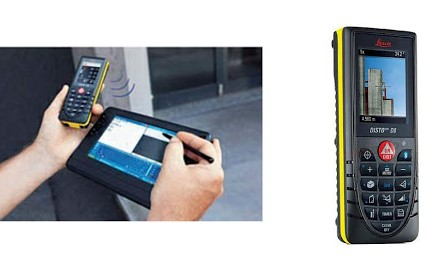
\includegraphics[scale=0.55]{images/instrument1.jpg} \hspace{2cm}
		\caption{Distancemètre laser Leica DISTO D8.\label{fig-instrument1}}
  	\end{center}
\end{figure}

 Parmi ses caractéristiques techniques, on peut citer:
	\begin{itemize}
		\item Une porté allant de 0.05m jusqu'à 200m.
		\item Une précision de $\pm 1mm$.
		\item Des opérations arithmétiques ainsi que des fonctions mathématiques sont intégrées à l'instrument telles que la fonction Pythagore, la fonction Trapèze ou encore la fonction triangle.
		\item Image en temps réel 
		\item Un Plug-In d'AutoCAD embarqué dans l'appareil qui permet de dessiner et de planifier avec le logiciel d'AutoCAD.
		\item Il inclut un logiciel de transfert de données pour le distancemètre  \textbf{Leica Disto Transfert}.
		\item Avec la technologie Bluetooth intégrée, l'utilisateur peut transférer les mesures effectuées vers un ordinateur portable ou un PC sans avoir recours aux câbles. Les données ainsi transférées peuvent être éditées à l'aide de logiciels tels que Word, Excel, AutoCAD, ....
	\end{itemize}
\end{description}

\begin{description}
	\item[Odomètre vérifiable PCE-MW 2]: Instrument permettant de mesurer différentes zones (ie: chantiers, zones industrielles, zones sportives, ...), des câblages, des tuyauteries, ....
\begin{figure}[H]
  %\centering
 	\begin{center}
 		\hspace{2cm}
		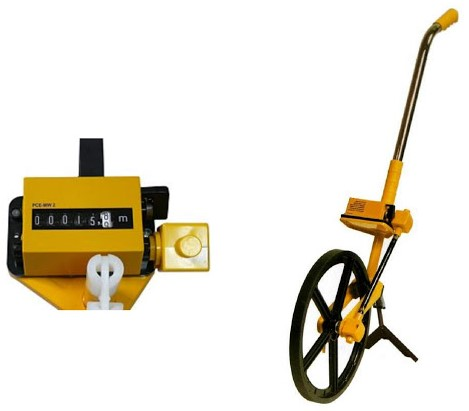
\includegraphics[scale=0.5]{images/instrument2.jpg} \hspace{2cm}
		\caption{Odomètre vérifiable PCE-MW 2.\label{fig-instrument2}}
  	\end{center}
\end{figure}
Parmi ses caractéristiques, on peut mentionner:
	\begin{itemize}
		\item Un poids de 2200g
		\item Mesure pouvant aller jusqu'à 99999,9 mètres.
		\item Permet d'effectuer une addition en se déplaçant vers l'avant et une soustraction en bougeant vers l'arrière.
		\item Une précision de $\pm 1\%$
		\item La roue est en plastique et permet de résister aux huiles.
	\end{itemize}	
\end{description}

\begin{description}
	\item[Distancemètre laser PCE-LRF 600]: Le design de cet instrument est bien conçu puisqu'il est léger et il permet de le maintenir avec une seule main. De plus, il est facile d'utilisation. 
\begin{figure}[H]
  %\centering
 	\begin{center}
 		\hspace{2cm}
		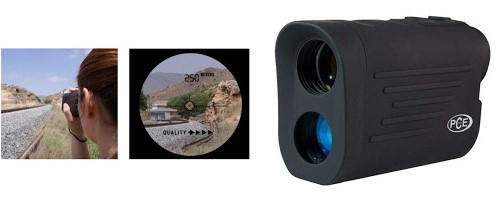
\includegraphics[scale=0.65]{images/instrument3.jpg} \hspace{2cm}
		\caption{Distancemètre laser PCE-LRF 600.\label{fig-instrument3}}
  	\end{center}
\end{figure}
De ses caractéristiques, on peut évoquer:
	\begin{itemize}
		\item Un poids de 165g.
		\item Une porté allant de 15m à 600m.
		\item Une précision de $\pm 1m/\pm 0.1\%$.
		\item Un laser de type classe 1.
		\item Une résistance aux éclaboussures d'eau
		\item Une mesure des distances dans diverses situations météorologiques.
	\end{itemize}
	
\end{description}


\subsection{Mesure d'erreurs par une approche théorique}
À ce jour, on recense de multiples méthodes exploitées à cet effet. Nous nous contentons de citer ci-dessous celles qui nous paraissent êtres les plus pertinentes. \\

\begin{description}
	\item[RMSE/RMSD]: Root Mean Square Error ou encore Root Mean Square Deviation que l'on pourrait traduire par; la racine carré de la moyenne des erreurs au carré. Elle demeure parmi les plus fréquentes en la matière. C'est une mesure de l'exactitude, qui permet de comparer les erreurs de prévision de différents modèles pour un ensemble de données précis et non entre des ensembles de données. Sa formule s'exprime comme suit:
	\begin{equation}
		\sqrt{\frac{1}{N}.\sum_{i = 1}^{N}(x_i - \hat{x_i})^2}
	\end{equation}	
De par la formule, on peut déduire que le résultat sera toujours positif et qu'obtenir une valeur de 0 (qui n'est généralement non atteint en pratique), témoignerait d'une exactitude parfaite. Ainsi, obtenir des valeurs avoisinant le zéro est positif pour les mesures.
	\item[MSE]: Mean Square Error que l'on pourrait traduire par; l'erreur quadratique moyenne. Sa formule est comme suit:
	\begin{equation}
		\frac{1}{N}.\sum_{i = 1}^{N}(x_i - \hat{x_i})^2
	\end{equation}
	
	\item[MAE]: Mean Absolute Error qui pourrait être traduit par; erreur moyenne absolue. Son équation est comme ci-dessous:
	\begin{equation}
		\frac{1}{N}.\sum_{i = 1}^{N} \abs{x_i - \hat{x_i}}
	\end{equation}	 
	\item[MAPE]: Mean Absolute Percentage Error qui pourrait être traduit par; le pourcentage de l'erreur moyenne absolue. Elle fait partie également des moyens de mesure d'erreurs les plus fréquents. A noter que la valeur observée ne doit être aucunement nulle. La formule est comme ci-après:
	\begin{equation}		
		\frac{1}{N}.\sum_{i = 1}^{N} \abs{\frac{x_i - \hat{x_i}}{x_i}}
	\end{equation}
\end{description}


Avec: \\ \\
$x_i$, la valeur observée à la ième observation. \\
$\hat{x}_i$, la valeur exacte à la ième observation. \\
$N$, le nombre d'observations.

%\section{Techniques existantes de capture de mouvements} 
\section[Technologies utilisées pour la depth]{Technologies utilisées pour la depth d'une caméra RGB-D} 
Des méthodes employées pour la récupération de la depth, on peut en citer deux principales.
\subsection{Infrarouge}
Le projecteur infrarouge de certaines caméras le possédant qu'on peut voir sur la figure \ref{fig-Asus} projette un spectre infrarouge sur la scène captée. Le motif produit sur cette dernière sera capté par la caméra infrarouge et sera par la suite comparé à la base de données de motifs de référence stockés au préalable dans la caméra. Ces derniers seront indispensables pour la mesure de la profondeur de chaque pixel. 

\begin{figure}[H]
  %\centering
 	\begin{center}
 		\hspace{-0.75cm}
		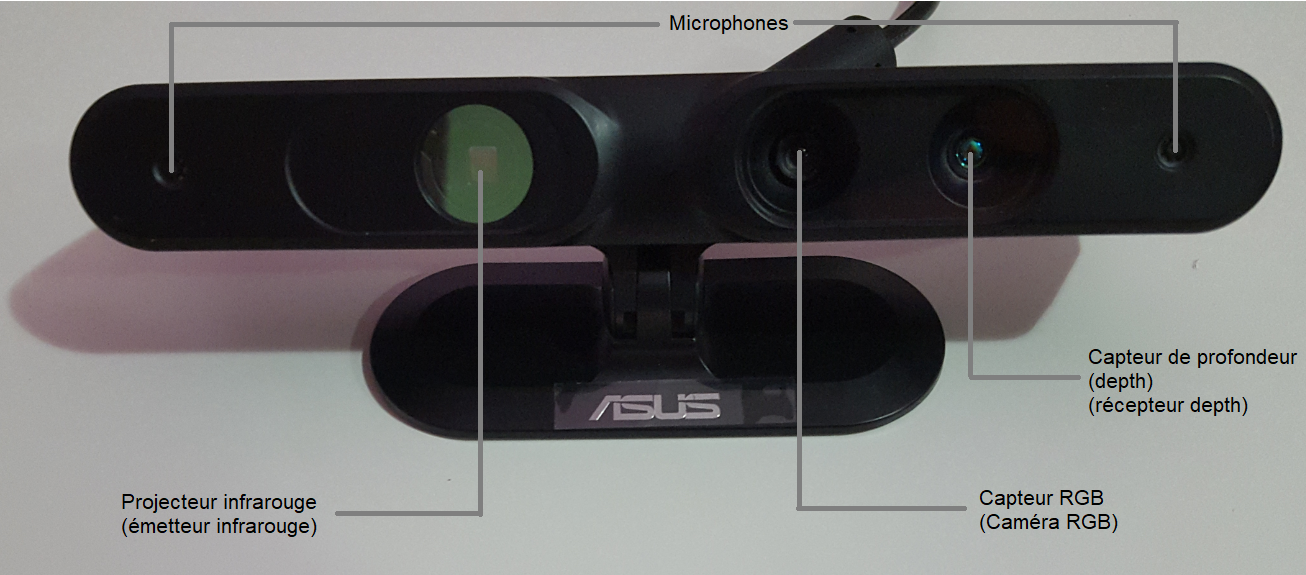
\includegraphics[scale=0.450]{images/Asus.png} \hspace{2cm}
		\caption{Composants caméra RGB-D (Ici Asus Xtion Pro Live).\label{fig-Asus}}
  	\end{center}
\end{figure}

Par la suite, les valeurs obtenues seront corrélées à un capteur RGB qu'on peut apercevoir sur la figure. Ces données pourront être représentées par un nuage de points \footnote{Est une représentation des points de coordonnées tridimensionnelles dont chacun peut avoir des attributs qui lui ont sont propres.}.


	\par Toutefois, ce type de caméras possède certaines restrictions. Parmi ces dernières, on peut citer:
	\begin{itemize}
		\item {Distances de mesure limitées.}	
		\item {Problèmes de calculs des informations de profondeur à l'encontre de surfaces brillantes, très mates, transparentes, réfléchissantes ou encore envers des objets absorbants.} 
		\item {Interférence des motifs (patterns) infrarouges si présence de plusieurs caméras RGB-D de même type. En effet, chaque capteur visualisera ses propres motifs ainsi que ceux des autres caméras présentes et ne saura distinguer les siens des autres qui se chevauchent.  De cela découle une perte considérable d'informations de profondeur comme nous pouvons l'observer sur la figure \ref{fig-interference}. 

\begin{figure}[H]
  %\centering
  \hspace{0.75cm}
 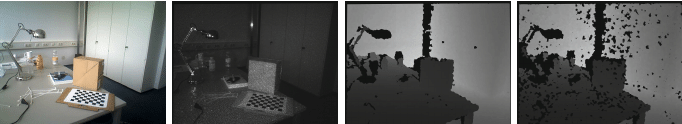
\includegraphics[scale=0.5]{images/interference.png}
  \caption{(De gauche à droite) image renvoyée par la caméra RGB, image IR, depth map (une seule caméra), depth map (deux caméras). (figure tirée de l'article de \emph{F.Alhwarin, A.Ferrein} et \emph{I.Scholl} ayant comme titre \emph{IR Stereo Kinect: Improving Depth Images by Combining StructuredLight with IR Stereo}).\label{fig-interference}}
\end{figure}

Cependant, des travaux de recherches ont été conduits afin d'y remédier. Parmi eux, on peut citer le travail réalisé par l'équipe de \emph{Rafibakhsh} ( \cite{RAFIBAKHSH15}) qui recommande de laisser un angle de 35\textdegree{} entre deux caméras suspendues à la même hauteur en considérant les scènes captées dans de bonnes conditions et une interférence très faible. \emph{Maimone} et \emph{Fuchs} \cite{MaimoneFuchs15} proposent un algorithme de remplissage et de lissage en modifiant le filtre médian aux zones trouées à l'exception des bords. Quant à \emph{F. Kenton Musgrave, Craig E.} et \emph{Robert S. Mace} \cite{KentonCraigMace12}, ils appliquent une certaine quantité minime de mouvements (en utilisant des composants matériels supplémentaires) à certains capteurs de sorte que chacun puisse voir son propre motif infrarouge de façon nette et une version floue des motifs de ses voisins. }
	\end{itemize}
\subsection{Stéréo-vision}
Une caméra stéréoscopique est un appareil qui contient deux voire plus de capteurs d'images. Ceci nous rappelle la vision binoculaire humaine. En effet, ce mécanisme permet au système nerveux central de percevoir simultanément les images issus de chaque œil envoyées sous forme de signaux. Ainsi, il sera en mesure de se servir de ces différences (entre les deux images)  pour permettre une vision stéréoscopique pour la perception de relief et une mesure des distances en utilisant la triangulation \footnote{Approche géométrique permettant une mesure des distances. Le lecteur peut consulter cette page web pour de plus amples informations: \url{https://fr.wikipedia.org/wiki/Triangulation} .}. Le concept que nous venons d'expliquer est appelé disparité stéréoscopique \footnote{Différence dans la localisation d'un objet perçu par l'œil gauche et l'œil droit résultant de la séparation horizontale des yeux dont certaines caméras essaient de s'approprier la technique afin de récupérer la profondeur.}. 
\par La stéréo-vision sert principalement à reconstituer la scène observée sous forme de modèle 3D. 
\subsubsection{Carte de disparités}
Le principe de la disparité est une approche du mécanisme humain vu précédemment. Il consiste en la différence entre les coordonnées pixels d'un point bidimensionnel d'une image et celles de son correspondant (présent sur une autre image prise au même moment). Ainsi, en appliquant le même traitement sur tous les pixels correspondants, on obtient la carte des disparités. Une carte est dite éparse lorsqu'une disparité est associée à quelques pixels et lorsque cette dernière est associée à chaque pixel, on dit d'elle qu'elle est dense.  \\ Une formule pour calculer la profondeur en fonction de la disparité s'obtient comme suit:
\begin{equation}
 z = \dfrac{B.f}{d}  
\end{equation} 
\\ Avec: \\ \\
$z$ représentant la profondeur. \\
$B$ \emph{Baseline} représente la distance séparant les deux capteurs. \\
$f$ La distance focale en pixels calculée comme montré ci-après en nous servant de la figure \ref{fig-focal} . \\
\begin{figure}[H]
  %\centering
  \hspace{-3cm}
 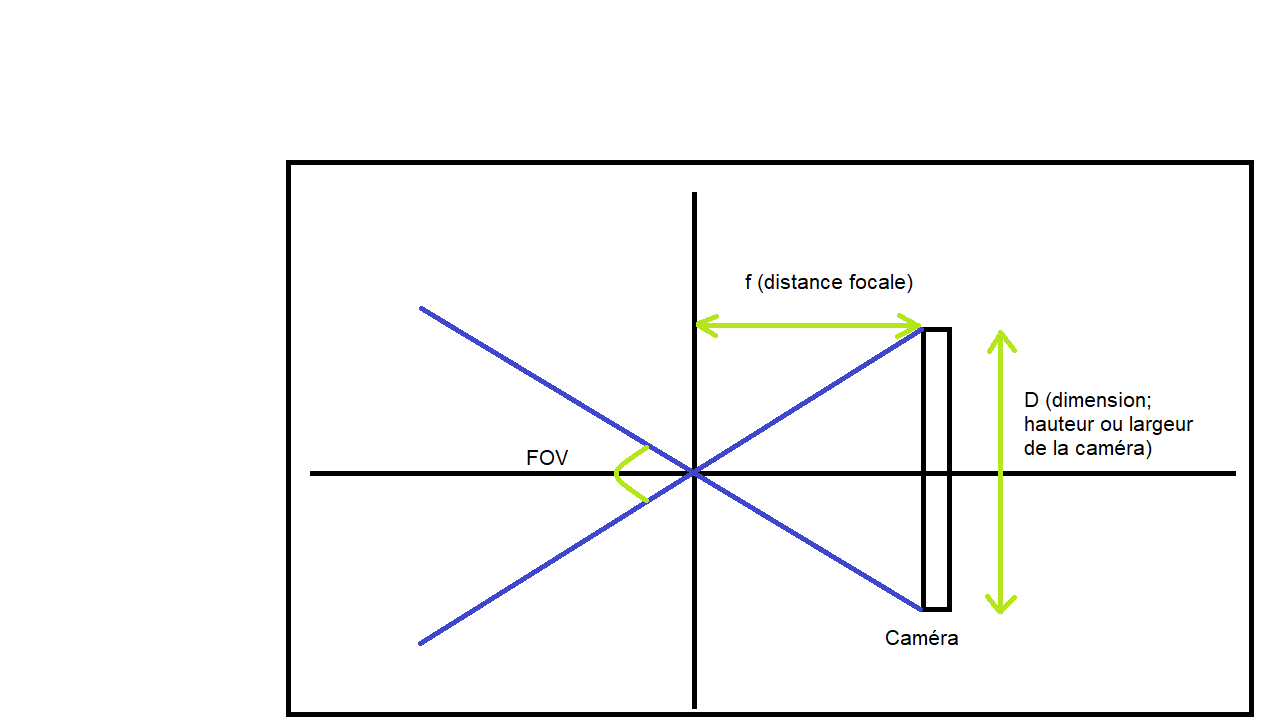
\includegraphics[scale=0.5]{images/focalLength.png} \hspace{2cm}
  \caption{Schéma illustrant la relation entre la distance focale et le champ de vision (fov).\label{fig-focal}}
\end{figure}


\begin{equation}
 \tan \left( {\dfrac{fov}{2}}\right) = \dfrac{D}{2.f}    \Leftrightarrow   f = \dfrac{D}{2. \tan \left( {\dfrac{fov}{2}}\right)}
\end{equation}
Avec:\\ \\
$D$  dimension qui peut représenter soit la largeur soit la hauteur en fonction du fov de la caméra employé. \\
$fov$ (Field Of View) représente l'angle du champ de vision (soit horizontal ou vertical). \\
$f$ représente la distance focale.


\section{Kinect V2 et Kinect V3}
\subsection{Kinect V2}
\texttt{Kinect V2} se sert de la méthode TOF (ie: Time Of Flight ou autrement dit Temps De Vol) pour générer la carte de profondeur. Cette technique se base sur la différence de temps entre l'émission d'un faisceau lumineux et son retour après réflexion sur un objet. \\ La distance est calculée comme suit:\\
$ d = c.\dfrac{\Delta t}{2} $, avec $c$ la vitesse de la lumière dans l'air.\\ \par Elle permet une bien meilleure précision même dans le noir que sa version précédente (\texttt{Kinect V1)}. 

\subsection{Kinect V3}
\texttt{Kinect V3}, baptisée \texttt{Microsoft Azure Kinect V3}, tout comme la précédente version, se base aussi sur la technologie TOF. Elle comprend un capteur RGB de 12 Mp, un capteur de depth de 1Mp avec un fov réglable en large ou réduit ainsi que 7 microphones intégrés.  
 
\subsubsection{Kinect V2 Vs Kinect V3}
\texttt{Kinect V3} est beaucoup plus légère et plus petite que la \texttt{V2}. Elle possède entre autre plus de microphones que la précédente. Elle a été conçue afin d'être principalement utilisée avec Azure , le service cloud de \texttt{Microsoft}. C'est sans doute ce qui la démarque le plus de sa prédécesseure. En effet, ce service lui permet d'effectuer une partie des calculs. En outre, elle bénéficie des Cognitive Services, autrement dit de l'intelligence artificielle pourra être incluse dans les applications créées.


\chapter[Modèle logiciel pour la qualification]{Modèle logiciel pour la qualification de caméra RGB-D}
Dans ce passage, nous allons décrire notre outil que nous avons pu concevoir pour qualifier les caméras.


\section{Description de l'application}

\begin{center}
	\begin{figure}[H]
  		\hspace{0.1cm}
 		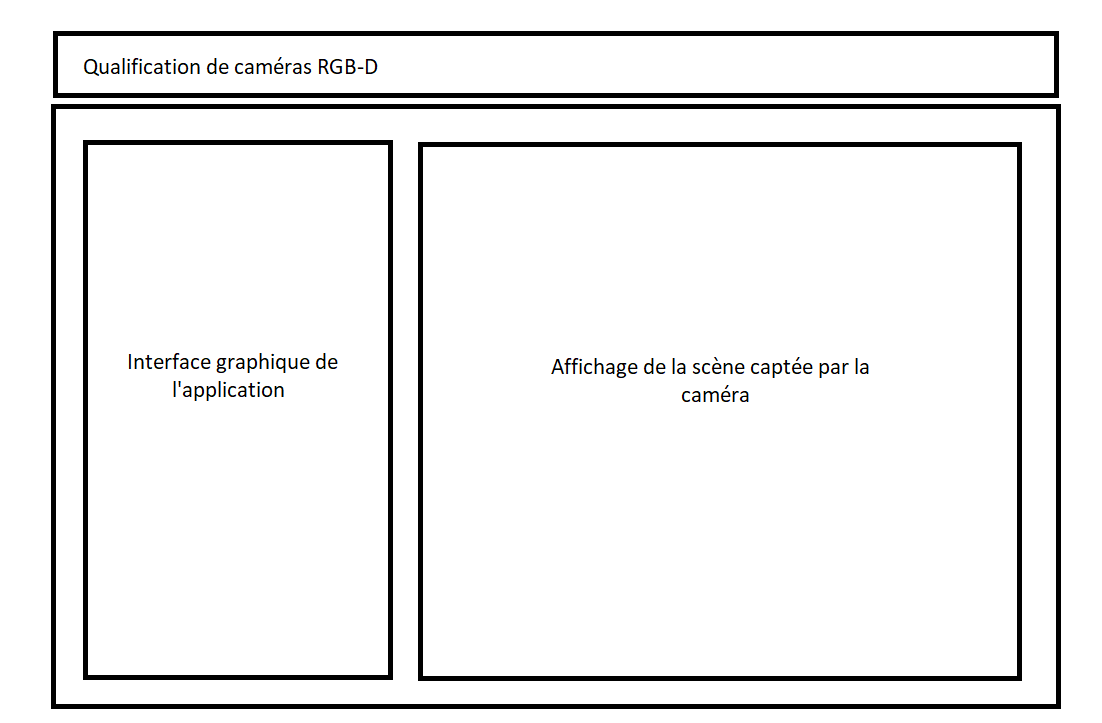
\includegraphics[scale=0.5]{images/maquetteApp1.png} \hspace{2cm}
  		\caption{Maquette globale de l'application.\label{fig-maquette}}
	\end{figure}
\end{center}

La figure \ref{fig-maquette} représente l'esquisse globale de l'application mise en œuvre. 

\begin{center}
	\begin{figure}[H]
  		\hspace{-1.5cm}
 		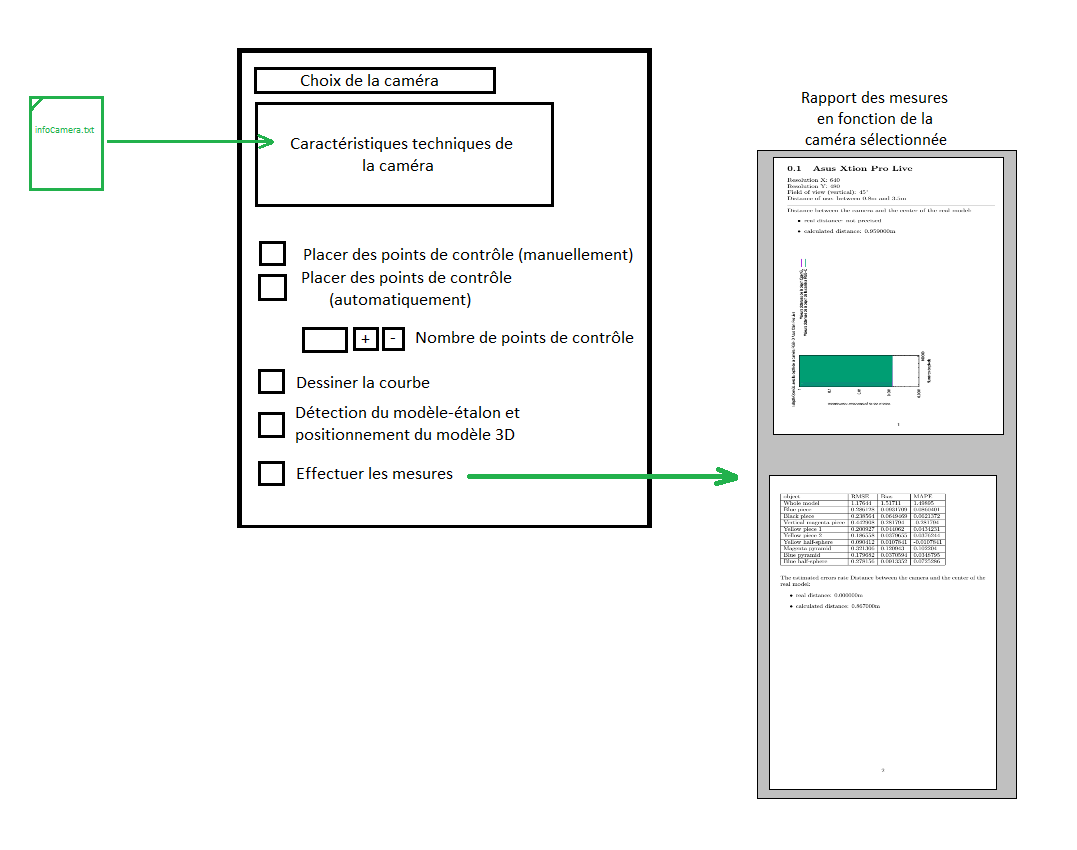
\includegraphics[scale=0.5]{images/maquetteApp2.png} \hspace{2cm}
  		\caption{Maquette de l'interface graphique de l'application.\label{fig-interface}}
	\end{figure}
\end{center}

La figure \ref{fig-interface} expose le squelette de l'interface graphique avec ses éléments la composant.

\section{Application développée}
Notre application est composée d'une fenêtre qui comprend une partie affichage de la scène filmée en temps réel ainsi qu'une partie interface graphique qui nous permet d'interagir avec le programme. Nous parlerons un peu plus en détail de ces parties dans les sous-sections à venir.
\subsection{Première partie: Affichage de la scène captée }
Pour cet effet, nous sommes partis d'un programme fourni par \emph{M. Farès BELHADJ} que nous avons complété par d'autres lignes de code pour la conception de l'outil. Il comprend l'utilisation de la bibliothèque OpenGL, GL4Dummies ainsi que la bibliothèque OpenNI2 pour établir la connexion avec la caméra RGB-D pour nous fournir par la suite la carte de couleurs et la carte de profondeurs. 
\subsection{Seconde partie: Interface graphique}
Pour l'interface graphique, nous avons exploité la bibliothèque Dear ImGui disponible sur GitHub sur le lien suivant \url{https://github.com/ocornut/imgui}. C'est une bibliothèque assez facile d'utilisation une fois l'étape de l'intégration dans le contexte OpenGL effectué. Cette interface contient un certain nombre de composants. Parmi les composants principaux, nous pouvons citer une liste déroulante qui nous permet de sélectionner le modèle de caméra sur laquelle nous souhaitons réaliser les tests de mesures. Ainsi, une fois le choix de caméra effectué, le programme met automatiquement à jour tous les paramètres présents dans les champs suivants la liste en récupérant les données à partir d'un fichier que nous avons nommé \emph{infoCameras.txt}. Ainsi, ce dernier pourra être exploité pour tout rajout de nouvelles caméras et/ou modification sur les données uniquement.
Autres les composants cités ci-dessus, nous noterons la présence de deux cases à cocher comme montré dans la figure \ref{fig-gui}. La première permet une détection du modèle et l'autre de passer les tests de mesures. Ces étapes seront détaillées dans les sous-sections à venir. 

\begin{center}
	\begin{figure}[H]
	 % \centering
	  \hspace{3cm}
	 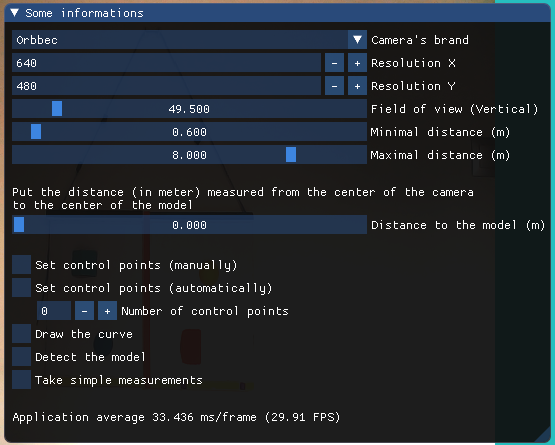
\includegraphics[scale=0.385]{images/GUI.png}
	  \caption{Interface graphique du programme.\label{fig-gui}}
	\end{figure}
\end{center}


\subsubsection{Détection du modèle réel}  

Pour cette partie, une fonction \emph{detectObject} est prévu à cet effet afin de renvoyer la localisation du modèle réel ainsi que celles des éléments le composant (demi-sphères, "pyramides", ...), ce qui fait un total de 10 objets à identifier. Une base de données d'images est crée pour servir de templates (images modèles) afin de pouvoir les distinguer. \par Pour chacun d'entre eux, un appel à la fonction \emph{callMatchTemplate} est effectué, qui, comme son nom l'indique, appelle la fonction \emph{matchTemplate} \footnote{Fonction OpenCV permettant de trouver à partir d'une image source les zones de correspondances avec l'image \emph{template}(image modèle). La documentation sur cette fonction est disponible sur le lien suivant: \url{https://docs.opencv.org/2.4/doc/tutorials/imgproc/histograms/template_matching/template_matching.html}}. Dans cette dernière, nous transformons notre image source (image récupérée de la scène captée par la caméra RGB-D) ainsi que notre image template en niveaux de gris et ensuite nous les passons sous le filtre Canny afin de rehausser les contours pour une meilleure détection \footnote{Nous nous sommes fortement inspirés du travail réalisé par Adrian ROSEBROCK, Ph.D en vision par ordinateur, disponible sur le lien suivant: \url {https://www.pyimagesearch.com/2015/01/26/multi-scale-template-matching-using-python-opencv/}.}. Ce processus qui comprend l'utilisation des filtres est appliqué uniquement pour la détection du model en entier et non sur ses composants. En effet, la couleur importe pour ces derniers puisque la forme n'est pas unique (présence de deux demi-sphères, ...).
\par Cette étape est assez conséquente en terme de temps. En effet, suivant la distance à laquelle est éloignée la caméra du modèle réel, le programme doit redimensionner la scène filmée avec une certaine échelle et avec un nombre précis de fois avant d'appeler la fonction \emph{matchTemplate}, qui, combinée avec \emph{minMaxLoc}\footnote{Fonction OpenCV qui renvoie les valeurs minimales et maximales d'une \emph{Mat}. Cette dernière est une sorte de vecteur ou plus communément une matrice.}, nous permet de renvoyer la localisation du modèle(coordonnées en $x$ et $y$ ainsi que la largeur et la hauteur de l'aire détectée). 
 De ce fait, une fois les coordonnées récupérées, nous pouvons positionner notre modèle virtuel dont nous discuterons les détails de conception un peu plus loin dans ce mémoire. Ces coordonnées seront naturellement converties en coordonnées OpenGL. La formule employée à cet effet (permettant une conversion d'un système de coordonnées vers un autre) est comme suit:\\ \\
$ value_{1} = \cfrac{value - min}{max - min}.(MAX - MIN) + MIN$ \\ \\ tel que $  value\in \left[min;max\right] $ (intervalle d'entrée) et $ value_{1}\in \left[MIN;MAX\right] $ (intervalle de sortie)  \\

\subsubsection{Tests de mesures et rédaction de rapport}
Pour celle-ci, nous récupérons les valeurs de la carte de profondeur d'OpenGL ainsi que les valeurs de profondeur de la caméra RGB-D. les valeurs de la depth OpenGL seront par la suite linéarisées \footnote{Technique employée pour \guillemotleft{}~ approcher par une fonction linéaire ~\guillemotright{}.} et ensuite normalisées \footnote{Standardiser les données afin qu'elles appartiennent à l'intervalle $ \left[0;1\right] $.}. Celles renvoyées par la caméra seront uniquement normalisées. Les valeurs des deux côtés étant normalisées, les tests de mesures peuvent débuter. \par Pour mesurer le taux d'erreur entre les valeurs des deux profondeurs, nous avons opté pour trois méthodes distinctes; RMSE \footnote{Root Mean Square Error est une méthode permettant de calculer l'écart-type des erreurs enregistrées. Se reférer à cette page web pour davantage de renseignements: \url{https://www.statisticshowto.datasciencecentral.com/rmse/}}, MAPE \footnote{Mean Absolute Percentage Error est une méthode permettant une mesure des erreurs tout comme le RMSE vu plus haut. Consulter cette page web pour un maximum d'informations: \url{https://www.statisticshowto.datasciencecentral.com/mean-absolute-percentage-error-mape/} } et enfin Biais \footnote{Tout comme les deux méthodes vu précédemment, elle permet un calcul du taux d'erreur. Le lecteur peut consulter ce lien la concernant \url{http://www.chups.jussieu.fr/polys/biostats/poly/POLY.Chp.10.html}}. Une fois ces valeurs calculées pour chacun des éléments du modèle ainsi que le modèle lui-même, nous les sauvegardons dans un tableau, tableau qui sera plus tard utilisé pour le rapport. \par Par la suite, nous nous servons de Gnuplot \footnote{Un logiciel multiplateforme gratuit qui offre la possibilité de tracer des graphes en deux ou trois dimensions.} afin de tracer les graphes montrant les valeurs de depth des deux côtés en faisant attention à ne pas écraser un éventuel graphe déjà présent. 
\par De plus, un rapport est rédigé en \LaTeX{} en mettant en avant les informations relatives à la caméra ( comme le champ de vision, la résolution, ...). A chaque fois qu'on coche sur la case \textit{Take simple measures} de l'interface graphique, le programme écrit ou réécrit sur un fichier que nous nommons \emph{Report.tex} situé dans un dossier \emph{Report} créé à cet effet. Si la caméra a déjà été testée, le programme rajoute dans la section la concernant(dans le rapport) les nouveaux résultats incluant graphe des valeurs de la depth, la distance calculée par le programme entre la caméra et le centre du modèle détecté ainsi qu'un tableau exposant les valeurs obtenues du taux d'erreurs pour les modèles et ses composants  avec les trois méthodes citées plus haut. Et ce, si et seulement si la caméra n'a pas été d'ores et déjà testée avec cette distance calculée par le programme.


\begin{figure}[htbp]
  %\centering
%  \hspace{5cm}
 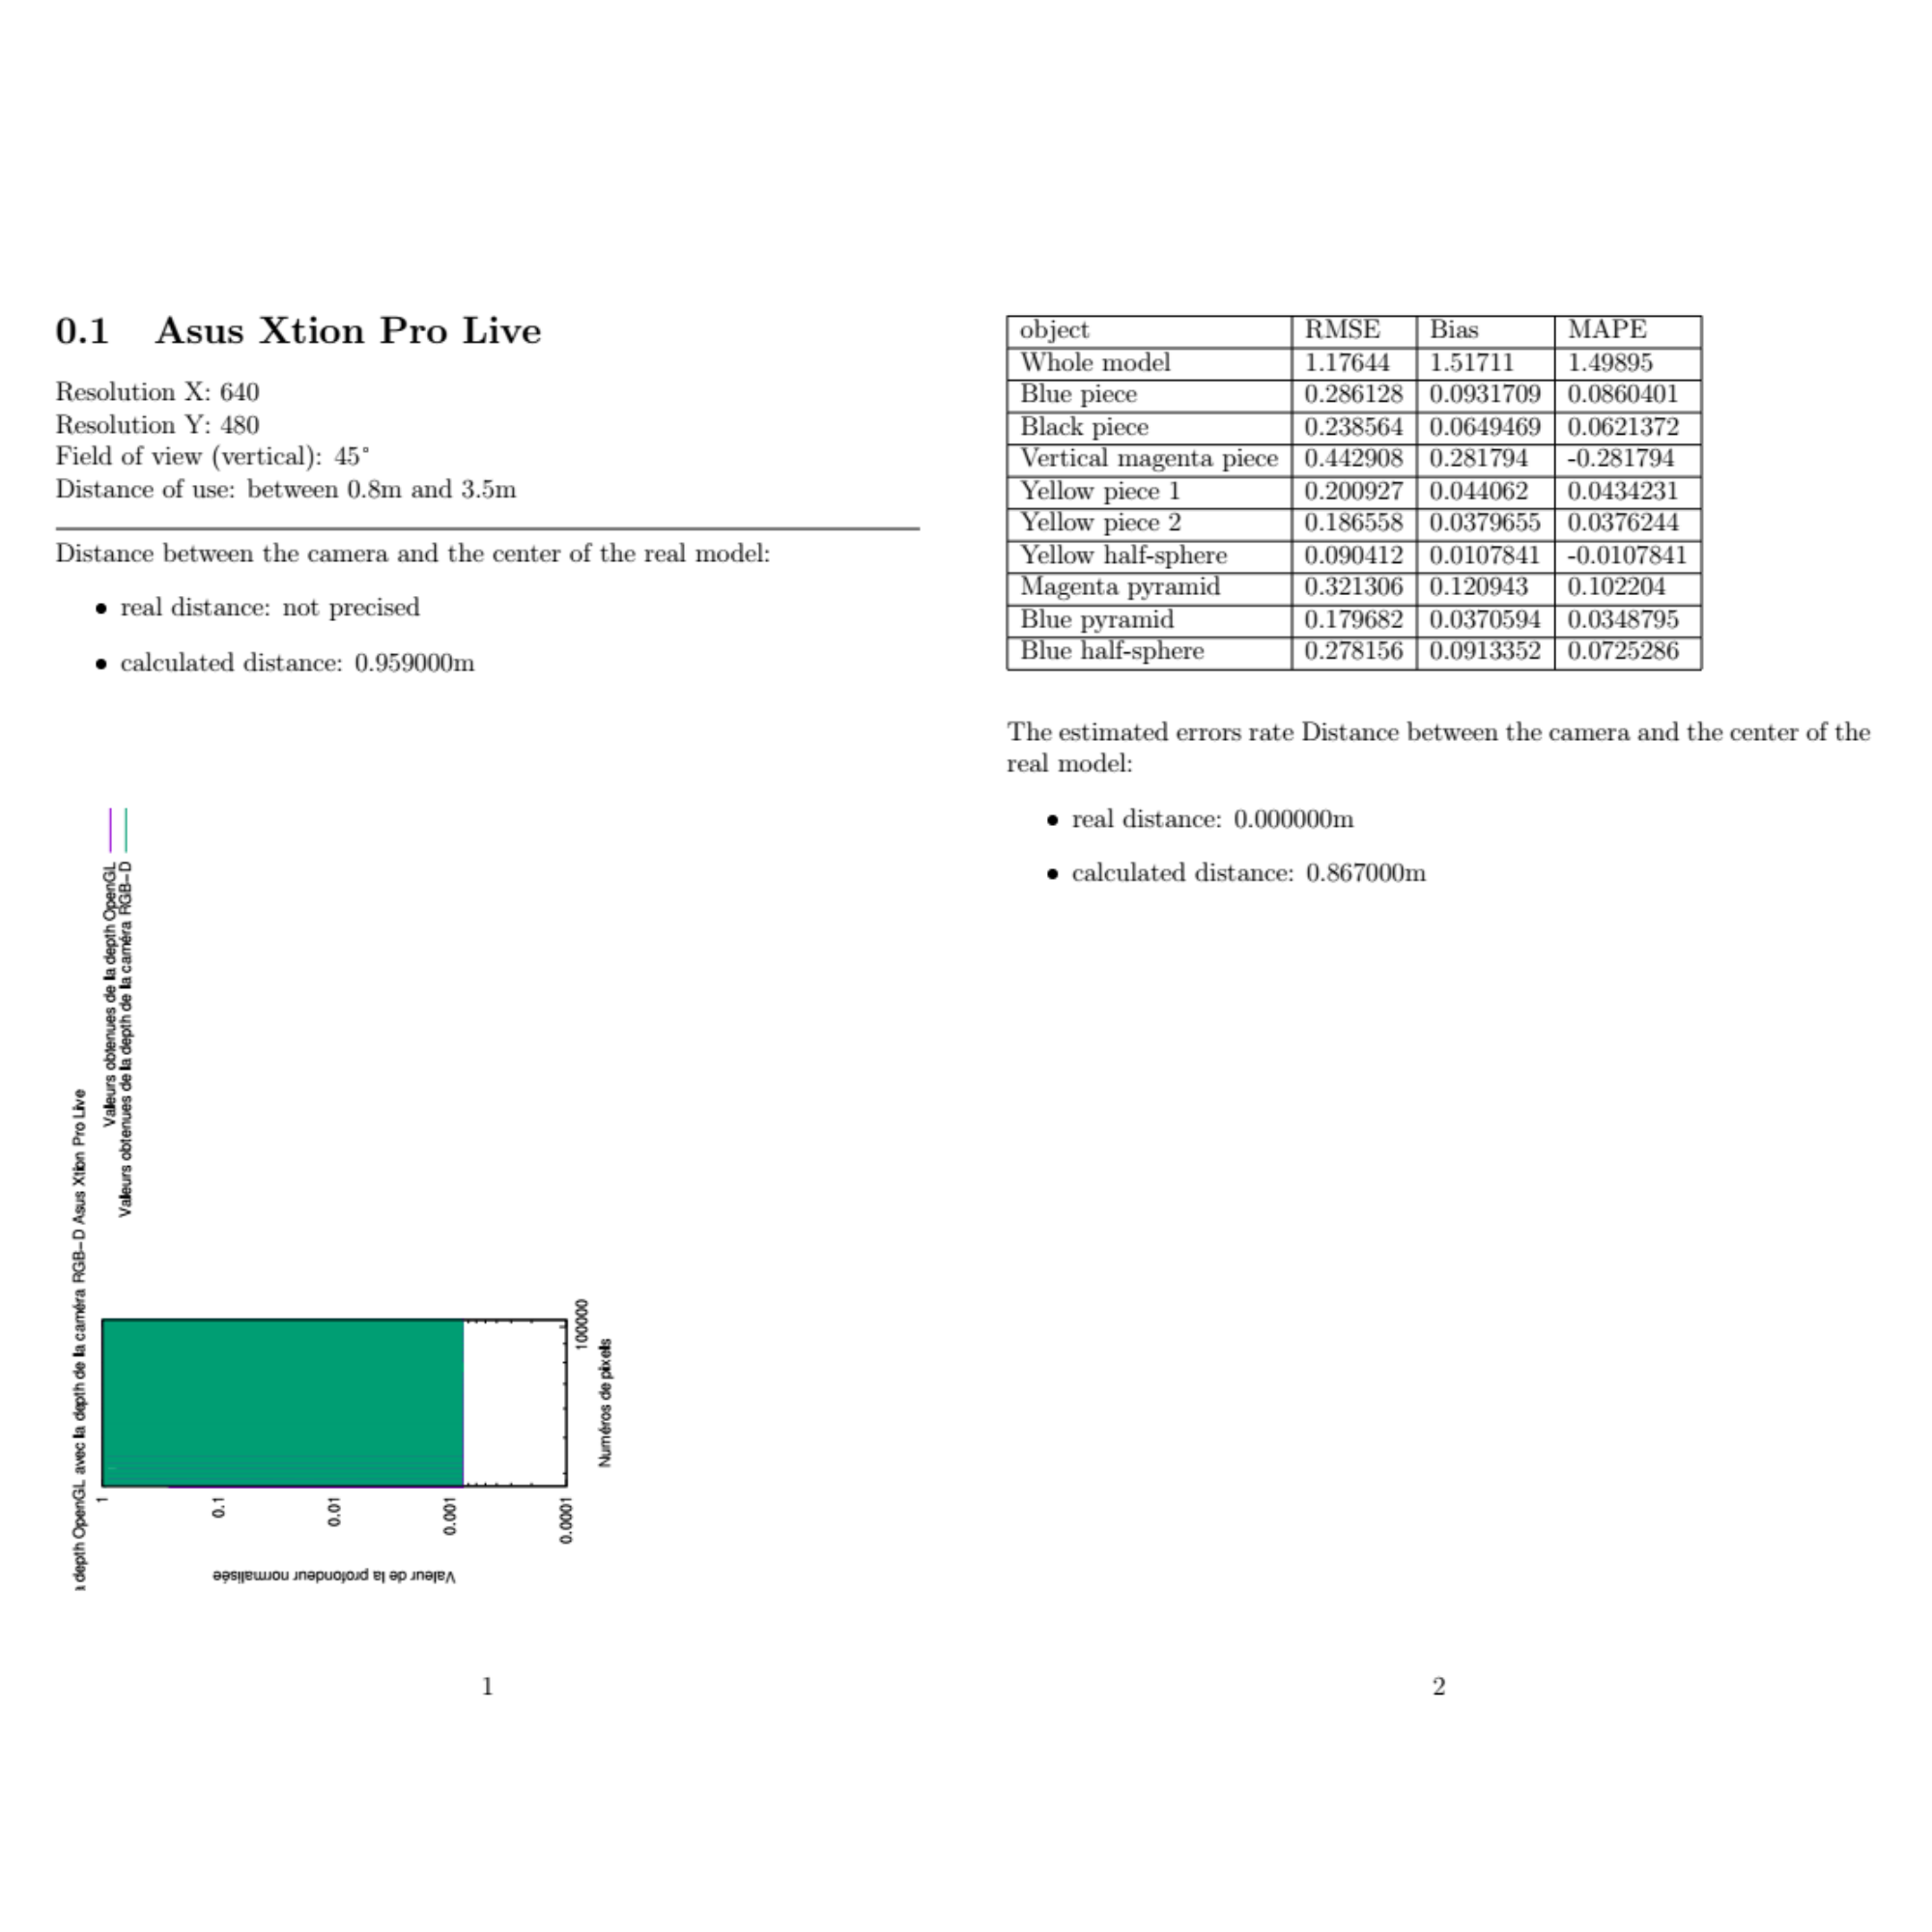
\includegraphics[scale=0.25]{images/report.png} \hspace{2cm}
  \caption{Partie du rapport généré par le programme.\label{fig-report}}
\end{figure}
\chapter{Cas pratiques de qualification}

\section{Conception du modèle réel et du modèle virtuel}
\subsection{Conception du modèle réel}
\begin{center}
	\begin{figure}[htbp]
  		\hspace{0.75cm}
 		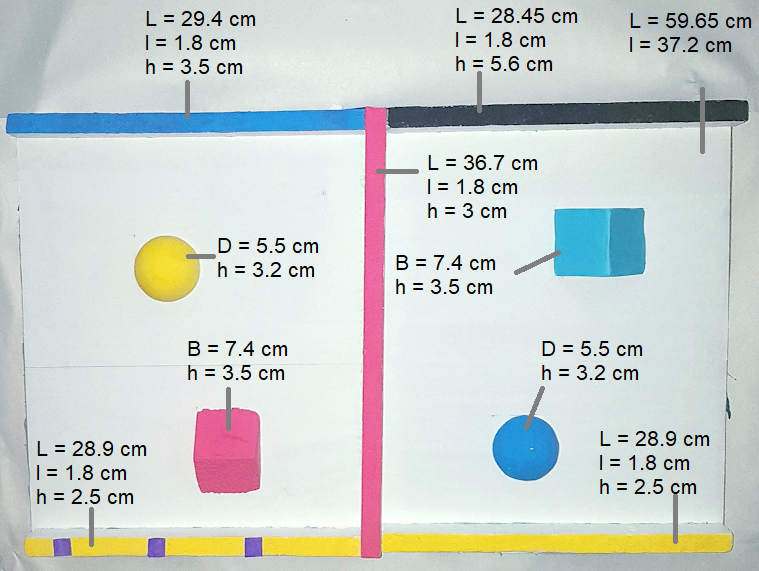
\includegraphics[scale=0.5]{images/realModel.png} \hspace{2cm}
  		\caption{Modèle-étalon.\label{fig-model}}
	\end{figure}
\end{center}

Pour fabriquer le modèle réel, nous avons décidé d'opter pour le polystyrène pour les composants du modèle et du carton pour sa base. Cette dernière sera par la suite recouverte de papier blanc. Les composants seront peints de couleurs distinctes suivant leur hauteur (les éléments qui possèdent une même hauteur seront peints de la même couleur plus particulièrement les rebords du modèle) sauf les demi-sphères et "pyramides".
\par Nous avons opté pour le polystyrène car c'est un matériau facilement maniable et que l'on peut trouver assez facilement. 
\subsection{Conception du modèle virtuel}
La réalisation du modèle virtuel s'est faite à l'aide du logiciel 123D Design qui est assez facile d'utilisation. Chaque élément du modèle est conçu en fonction des vraies mesures faites sur le modèle réel.
\begin{center}
	\begin{figure}[htbp]
  		\hspace{0.37cm}
 		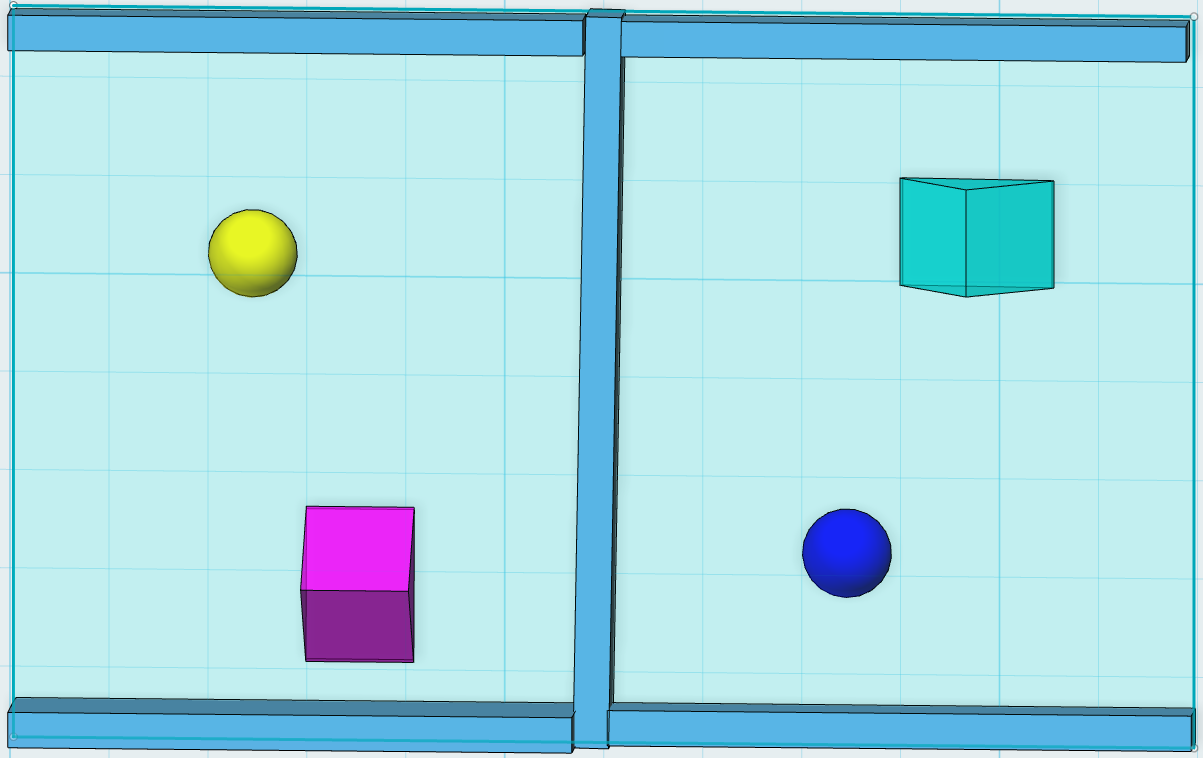
\includegraphics[scale=0.35]{images/3DModel.png} \hspace{2cm}
  		\caption{Modèle 3D.\label{fig-3Dmodel}}
	\end{figure}
\end{center}

\section{Preuve de concept (Proof of concept - POC)}
Dans cette section, nous exposons la procédure suivie pour configurer les caméras \texttt{Asus Xtion Pro Live} et \texttt{Orbbec Astra Pro} afin que le programme puisse procéder aux tests de mesures.
Tout d'abord, nous avons édité le fichier \emph{infoCameras.txt} cité dans le chapitre précédent en vue d'y rajouter les informations relatives à ces caméras.
\par Par la suite, nous n'avons pas eu besoin de rajouter des lignes de code pour la reconnaissance de la caméra \texttt{Asus Xtion Pro Live} (initialisation et récupération de la carte de couleurs et de la carte de profondeurs) car ce modèle est reconnu par la bibliothèque OpenNI2. Bien que la caméra \texttt{Orbbec Astra Pro} soit aussi supportée par cette bibliothèque, il a quand même été indispensable de rajouter des lignes de code afin de récupérer la carte de couleurs. En effet, OpenNI2 ne permet pas de la capturer, par conséquent, nous avons dû exploiter certains aspects de la bibliothèque OpenCV pour se faire.
\par Enfin, il nous suffira de sélectionner, à partir de l'interface de l'application, le modèle de la caméra branché et cocher sur les cases \emph{Detect the model} pour une détection du modèle-étalon et \emph{Take simple measures} pour démarrer les tests de mesures et la rédaction automatique du rapport comme expliqué précédemment. 


\section{Résultats et critique}
\subsection{Résultats obtenus}
Ces résultats sont extraits du rapport rédigé par le programme après réalisation des tests avec les caméras Asus Xtion Pro Live et Orbbec Astra Pro sur trois distances différentes exprimées en mètre (distance entre la caméra et le modèle). Nous avons créé la base de données d'images templates suivant une des distances.  \\ \\

\vspace{2cm}


\begin{table}[H]
\centering
\setlength\tabcolsep{2pt}
\begin{tabular}{c|lllllllll}
\cline{1-7}
\multicolumn{1}{|l|}{}   & 
\multicolumn{6}{l|}{\textbf{\hspace{3cm} Distances (m)}}    \\
\cline{1-7}
\multicolumn{1}{|l|}{\textbf{}}   & 
\multicolumn{2}{l|}{\textbf{1.7 }} & 
\multicolumn{2}{l|}{\textbf{1.609}} & 
\multicolumn{2}{l|}{\textbf{1.522}} &  \\

\cline{1-7}
\multicolumn{1}{|l|}{\textbf{object}}   & 
\multicolumn{1}{l|}{\textbf{Asus }} & 
\multicolumn{1}{l|}{\textbf{Orbbec}} & 
\multicolumn{1}{l|}{\textbf{Asus}} &  
\multicolumn{1}{l|}{\textbf{Orbbec }} & 
\multicolumn{1}{l|}{\textbf{Asus}} & 
\multicolumn{1}{l|}{\textbf{Orbbec}} & \\

\cline{1-7}
\multicolumn{1}{|l|}{Whole model}  & 
\multicolumn{1}{l|}{51\%}  &  
\multicolumn{1}{l|}{81\%}  & 
\multicolumn{1}{l|}{90\%}  & 
\multicolumn{1}{l|}{40\%}  & 
\multicolumn{1}{l|}{91\%}  & 
\multicolumn{1}{l|}{75\%}  &  \\ 
\cline{1-7}
\multicolumn{1}{|l|}{Blue piece}  &
\multicolumn{1}{l|}{55\%}  &
\multicolumn{1}{l|}{45\%}  & 
\multicolumn{1}{l|}{91\%} & 
\multicolumn{1}{l|}{50\%}  & 
\multicolumn{1}{l|}{94\%}  &  
\multicolumn{1}{l|}{41\%}  &   \\ 
\cline{1-7}
\multicolumn{1}{|l|}{Black piece}  & 
\multicolumn{1}{l|}{56\%}  & 
\multicolumn{1}{l|}{46\%}  & 
\multicolumn{1}{l|}{91\%} & 
\multicolumn{1}{l|}{50\%}  & 
\multicolumn{1}{l|}{94\%}  &
\multicolumn{1}{l|}{42\%}  &  \\ 
\cline{1-7}
\multicolumn{1}{|l|}{Vertical magenta piece}  & 
\multicolumn{1}{l|}{55\%}  & 
\multicolumn{1}{l|}{46\%}  & 
\multicolumn{1}{l|}{91\%} & 
\multicolumn{1}{l|}{50\%}  & 
\multicolumn{1}{l|}{94\%}  & 
\multicolumn{1}{l|}{41\%}  & \\ 
\cline{1-7}
\multicolumn{1}{|l|}{Yellow piece 1}  & 
\multicolumn{1}{l|}{28\%}  & 
\multicolumn{1}{l|}{98\%}  & 
\multicolumn{1}{l|}{93\%}  & 
\multicolumn{1}{l|}{22\%}  & 
\multicolumn{1}{l|}{99\%}  & 
\multicolumn{1}{l|}{97\%}  & \\ 
\cline{1-7}
\multicolumn{1}{|l|}{Yellow piece 2}  & 
\multicolumn{1}{l|}{28\%}  & 
\multicolumn{1}{l|}{98\%}  & 
\multicolumn{1}{l|}{94\%}  &  
\multicolumn{1}{l|}{48\%}  & 
\multicolumn{1}{l|}{99\%}  & 
\multicolumn{1}{l|}{97\%}  & \\ 
\cline{1-7}
\multicolumn{1}{|l|}{Yellow half-sphere}  & 
\multicolumn{1}{l|}{54\%}  & 
\multicolumn{1}{l|}{45\%}  & 
\multicolumn{1}{l|}{90\%}  &  
\multicolumn{1}{l|}{51\%}  & 
\multicolumn{1}{l|}{94\%}  & 
\multicolumn{1}{l|}{37\%}  & \\ 
\cline{1-7}
\multicolumn{1}{|l|}{Magenta pyramid}  & 
\multicolumn{1}{l|}{53\%}  & 
\multicolumn{1}{l|}{46\%}  & 
\multicolumn{1}{l|}{90\%}  &  
\multicolumn{1}{l|}{51\%}  & 
\multicolumn{1}{l|}{94\%}  & 
\multicolumn{1}{l|}{37\%}  & \\ 
\cline{1-7}
\multicolumn{1}{|l|}{Blue pyramid}  & 
\multicolumn{1}{l|}{53\%}  & 
\multicolumn{1}{l|}{46\%}  & 
\multicolumn{1}{l|}{91\%}  &  
\multicolumn{1}{l|}{50\%}  & 
\multicolumn{1}{l|}{94\%}  & 
\multicolumn{1}{l|}{38\%}  & \\ 
\cline{1-7}
\multicolumn{1}{|l|}{Blue  half-sphere}  & 
\multicolumn{1}{l|}{55\%}  & 
\multicolumn{1}{l|}{45\%}  & 
\multicolumn{1}{l|}{90\%}  &  
\multicolumn{1}{l|}{52\%}  & 
\multicolumn{1}{l|}{94\%}  & 
\multicolumn{1}{l|}{37\%}  & \\ 
\cline{1-7}
\multicolumn{1}{|l|}{\textbf{Average rate}} & 
\multicolumn{1}{l|}{\textbf{48.8\%}}  & 
\multicolumn{1}{l|}{\textbf{59.6\%}}  &  
\multicolumn{1}{l|}{\textbf{91.1\%}}  & 
\multicolumn{1}{l|}{\textbf{46.4\%}}  & 
\multicolumn{1}{l|}{\textbf{94.7\%}}  & 
\multicolumn{1}{l|}{\textbf{54.2\%}}  & \\ 
\cline{1-7}

\end{tabular}
\end{table}
\vspace{2cm} 
\par On peut aisément observer un taux d'erreur moins important avec la Orbbec.
Les taux restent néanmoins très élevés.

\subsection{Critiques}
\par Les taux anormalement élevés observés dans la section précédente nous prélèvent des doutes sur deux points principaux qui pourraient être omis dans l'application.
\begin{itemize}
		\item {Fiabilité des valeurs de la depth OpenGL extraites.}	
		\item {Aire de détection du modèle 3D non conforme à celle du modèle réel en terme de coordonnées.} 		
\end{itemize}

\par Pour l'heure, à moins que nous ignorons d'autres points, nous ne voyons pas d'autres éléments qui pourraient impacter ces résultats. 


\chapter{Conclusion et Perspectives\label{chap-conclusion}}
\par Dans ce rapport, nous avons présenté l'outil que nous avons développé à ce jour pour la qualification de caméras RGB-D. D'après les résultats exposés précédemment, nous pouvons admettre que la \texttt{Orbbec Astra Pro} l'emporte sur la \texttt{Asus Xtion Pro Live} en terme de précision dans la mesure. 
\par Cependant, comme nous avons pu le constater sur les deux caméras, cette application renvoyait des taux d'erreur excessivement élevés, ce qui nous a questionné sur sa fiabilité. Ainsi, nous avons établis deux éléments qui pourraient potentiellement être à l'origine de cette anomalie. 
\begin{itemize}
		\item {Fiabilité de la depth OpenGL.}	
		\item {Non conformité des coordonnées des zones détectées entre le modèle réel et le modèle virtuel.} 		
\end{itemize} 

\vspace{0.5cm}
\par En perspectives, nous souhaiterions vérifier de manière plus pointilleuse les données OpenGL extraites ainsi que la correspondance entre les deux aires de détection.
Dans ce cas, la qualification pourra être effectuée dans des conditions permettant une meilleure comparaison entre les différents modèles de caméras.  
\par Une fois les conditions réunies, nous pensons effectuer les tests de mesures sur la colonne vertébrale d'un vrai patient. Pour ce faire, il nous faut rechercher un modèle 3D de colonne vertébrale ou un modèle s'en rapprochant le plus possible. 	

\par L'application résultante devra être en mesure de détecter la colonne vertébrale de la personne posant de dos à la caméra RGB-D. Les personnes qui suscitent notre intérêt sont principalement ceux atteints de scoliose. Dans un premier lieu, la localisation de l'épine dorsale va être effectuée en se basant sur du Machine Learning. Par la suite, une fois la colonne vertébrale détectée, le programme devra être apte à bien positionner le modèle 3D de manière à ce qu'il corresponde à l'épine dorsale du patient observé. Enfin, les tests de mesures pourront être lancés.


\nocite{*}
\bibliographystyle{alpha}
\bibliography{memoire}
%\nocite{*}
%\bibliographystyle{unsrt}
%\bibliographystyle{alpha}

%\bibliography{memoire}
%\printbibliography

\end{document}

